
%(BEGIN_QUESTION)
% Copyright 2008, Tony R. Kuphaldt, released under the Creative Commons Attribution License (v 1.0)
% This means you may do almost anything with this work of mine, so long as you give me proper credit

Calculate the voltage magnitude and polarity between points {\bf A} and {\bf D} in this circuit, assuming a power supply output voltage of 10.5 volts:

$$\includegraphics[width=15.5cm]{i03150x01.eps}$$

Also, calculate the total current output by the power supply as it energizes this resistor network.  Be sure to show all your work!

\vfil 

\underbar{file i03150}
\eject
%(END_QUESTION)





%(BEGIN_ANSWER)

This is a graded question -- no answers or hints given!

%(END_ANSWER)





%(BEGIN_NOTES)

$V_{AD} = 7.31 \hbox{ volts}$, {\bf A} positive and {\bf D} negative.  The total power supply current is 4.36 mA.

%INDEX% Electronics review: series-parallel circuits

%(END_NOTES)


